In this section we will have a high level look on the algorithms that we are going to use.

\textbf{Random Schedule:}

\begin{itemize}

\item Places all VNFs on all nodes of the networks

\item Creates random schedules for each source node, each SFC, each SF , each destination node

\item All the schedules for an SF sum-up to 1

\end{itemize}


\textbf{Load Balance algorithm:}

\begin{itemize}

\item Always returns equal distribution for all nodes having capacities and SFs. Places all SFs on all nodes having some capacity.

\end{itemize}

\textbf{Shortest path algorithm:}

Based on network topology, SFC, and ingress nodes, calculates for each ingress node:
\begin{itemize}

\item Puts 1st VNF on ingress, 2nd VNF on closest neighbor, 3rd VNF again on closest neighbor of 2nd VNF and so on.

\item Stores placement of VNFs and avoids placing 2 VNFs on the same node as long as possible. If all nodes are filled, continue placing a 2nd VNF on all nodes, but avoid placing 3 VNFs and so on.

\item Avoids nodes without any capacity at all (but ignores current utilization).

\end{itemize}

\begin{figure}[h]
    \centering
    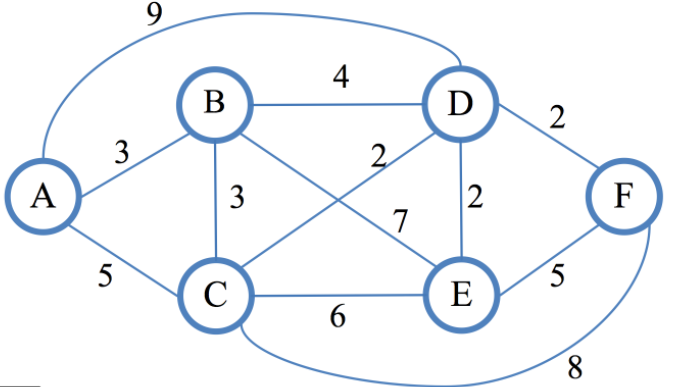
\includegraphics[width=1\textwidth]{shortesth path}
    \caption{Shortest path Algorithm}
    \label{fig:shortesth path}
\end{figure}